\ifx\wholebook\relax \else
% ------------------------ 

\documentclass{article}
%------------------- Other types of document example ------------------------
%
%\documentclass[twocolumn]{IEEEtran-new}
%\documentclass[12pt,twoside,draft]{IEEEtran}
%\documentstyle[9pt,twocolumn,technote,twoside]{IEEEtran}
%
%-----------------------------------------------------------------------------
%%
% loading packages
%
\newif\ifpdf
\ifx\pdfoutput\undefined % We're not running pdftex
  \pdffalse
\else
  \pdftrue
\fi
%
%
\ifpdf
  \RequirePackage[pdftex,%
            CJKbookmarks,%
       bookmarksnumbered,%
              colorlinks,%
          linkcolor=blue,%
              hyperindex,%
        plainpages=false,%
       pdfstartview=FitH]{hyperref}
\else
  \RequirePackage[dvipdfm,%
             CJKbookmarks,%
        bookmarksnumbered,%
               colorlinks,%
           linkcolor=blue,%
               hyperindex,%
         plainpages=false,%
        pdfstartview=FitH]{hyperref}
  \AtBeginDvi{\special{pdf:tounicode GBK-EUC-UCS2}} % GBK -> Unicode
\fi
\usepackage{hyperref}

% other packages
%-----------------------------------------------------------------------------
\usepackage{graphicx, color}
\usepackage{CJK}
%
% for programming 
%
\usepackage{verbatim}
\usepackage{listings}


\lstdefinelanguage{Smalltalk}{
  morekeywords={self,super,true,false,nil,thisContext}, % This is overkill
  morestring=[d]',
  morecomment=[s]{"}{"},
  alsoletter={\#:},
  escapechar={!},
  literate=
    {BANG}{!}1
    {UNDERSCORE}{\_}1
    {\\st}{Smalltalk}9 % convenience -- in case \st occurs in code
    % {'}{{\textquotesingle}}1 % replaced by upquote=true in \lstset
    {_}{{$\leftarrow$}}1
    {>>>}{{\sep}}1
    {^}{{$\uparrow$}}1
    {~}{{$\sim$}}1
    {-}{{\sf -\hspace{-0.13em}-}}1  % the goal is to make - the same width as +
    %{+}{\raisebox{0.08ex}{+}}1		% and to raise + off the baseline to match -
    {-->}{{\quad$\longrightarrow$\quad}}3
	, % Don't forget the comma at the end!
  tabsize=2
}[keywords,comments,strings]

\lstloadlanguages{C++, Lisp, Haskell, Python, Smalltalk}

% ======================================================================

\def\BibTeX{{\rm B\kern-.05em{\sc i\kern-.025em b}\kern-.08em
    T\kern-.1667em\lower.7ex\hbox{E}\kern-.125emX}}

\newtheorem{theorem}{Theorem}

%
% mathematics
%
\newcommand{\be}{\begin{equation}}
\newcommand{\ee}{\end{equation}}
\newcommand{\bmat}[1]{\left( \begin{array}{#1} }
\newcommand{\emat}{\end{array} \right) }
\newcommand{\VEC}[1]{\mbox{\boldmath $#1$}}

% numbered equation array
\newcommand{\bea}{\begin{eqnarray}}
\newcommand{\eea}{\end{eqnarray}}

% equation array not numbered
\newcommand{\bean}{\begin{eqnarray*}}
\newcommand{\eean}{\end{eqnarray*}}

\RequirePackage{CJK,CJKnumb,CJKulem,CJKpunct}
% we use CJK as default environment
\AtBeginDocument{\begin{CJK*}{GBK}{song}\CJKtilde\CJKindent\CJKcaption{GB}}
\AtEndDocument{\clearpage\end{CJK*}}

%
% loading packages
%

\RequirePackage{ifpdf}

%
%
\ifpdf
  \RequirePackage[pdftex,%
       bookmarksnumbered,%
              colorlinks,%
          linkcolor=blue,%
              hyperindex,%
        plainpages=false,%
       pdfstartview=FitH]{hyperref}
\else
  \RequirePackage[dvipdfm,%
        bookmarksnumbered,%
               colorlinks,%
           linkcolor=blue,%
               hyperindex,%
         plainpages=false,%
        pdfstartview=FitH]{hyperref}
\fi
\usepackage{hyperref}

% other packages
%--------------------------------------------------------------------------
\usepackage{graphicx, color}
\usepackage{subfig}

\usepackage{amsmath, amsthm, amssymb} % for math
\usepackage{exercise} % for exercise

%
% for programming 
%
\usepackage{verbatim}
\usepackage{listings}
%\usepackage{algorithmic} %old version; we can use algorithmicx instead
\usepackage{algorithm} 
\usepackage[noend]{algpseudocode} %for pseudo code, include algorithmicsx automatically
\usepackage{makeidx} % for index support


\lstdefinelanguage{Smalltalk}{
  morekeywords={self,super,true,false,nil,thisContext}, % This is overkill
  morestring=[d]',
  morecomment=[s]{"}{"},
  alsoletter={\#:},
  escapechar={!},
  literate=
    {BANG}{!}1
    {UNDERSCORE}{\_}1
    {\\st}{Smalltalk}9 % convenience -- in case \st occurs in code
    % {'}{{\textquotesingle}}1 % replaced by upquote=true in \lstset
    {_}{{$\leftarrow$}}1
    {>>>}{{\sep}}1
    {^}{{$\uparrow$}}1
    {~}{{$\sim$}}1
    {-}{{\sf -\hspace{-0.13em}-}}1  % the goal is to make - the same width as +
    %{+}{\raisebox{0.08ex}{+}}1		% and to raise + off the baseline to match -
    {-->}{{\quad$\longrightarrow$\quad}}3
	, % Don't forget the comma at the end!
  tabsize=2
}[keywords,comments,strings]

\lstloadlanguages{C++, Lisp, Haskell, Python, Smalltalk}

% ======================================================================

\def\BibTeX{{\rm B\kern-.05em{\sc i\kern-.025em b}\kern-.08em
    T\kern-.1667em\lower.7ex\hbox{E}\kern-.125emX}}

%
% mathematics
%
\newcommand{\be}{\begin{equation}}
\newcommand{\ee}{\end{equation}}
\newcommand{\bmat}[1]{\left( \begin{array}{#1} }
\newcommand{\emat}{\end{array} \right) }
\newcommand{\VEC}[1]{\mbox{\boldmath $#1$}}

% numbered equation array
\newcommand{\bea}{\begin{eqnarray}}
\newcommand{\eea}{\end{eqnarray}}

% equation array not numbered
\newcommand{\bean}{\begin{eqnarray*}}
\newcommand{\eean}{\end{eqnarray*}}

\newtheorem{theorem}{Theorem}[section]
\newtheorem{lemma}[theorem]{Lemma}
\newtheorem{proposition}[theorem]{Proposition}
\newtheorem{corollary}[theorem]{Corollary}


\setcounter{page}{1}

\begin{document}

\fi
%--------------------------

% ================================================================
%                 COVER PAGE
% ================================================================

\title{Binomial heap, Fibonacci heap, and pairing heap}

\author{Liu~Xinyu
\thanks{{\bfseries Liu Xinyu } \newline
  Email: liuxinyu95@gmail.com \newline}
  }

\markboth{Binomial heap, Fibonacci heap, and pairing heap}{AlgoXY}

\maketitle

\ifx\wholebook\relax
\chapter{Binomial heap, Fibonacci heap, and pairing heap}
\fi

% ================================================================
%                 Introduction
% ================================================================
\section{Introduction}
\label{introduction}
In previous chapter, we mentioned that heaps can be
generalized and implemented with varies of data structures. However,
only binary heaps are focused so far no matter by explicit binary
trees or implicit array. 

It's quite natural to extend the binary tree to K-ary \cite{K-ary-tree} tree. 
In this chapter, we first show Binomial heaps 
which is actually consist of forest of K-ary trees. Binomial heaps gain the 
performance for all operations to $O(\lg N)$, as well as keeping the finding 
minimum element to $O(1)$ time.

If we delay some operations in Binomial
heaps by using lazy strategy, it turns to be Fibonacci heap.
 
All binary heaps we have shown perform
no less than $O(\lg N)$ time for merging, we'll show it's possible to 
improve it to $O(1)$ with Fibonacci heap, which is quite helpful to 
graph algorithms. Actually, Fibonacci heap acheives almost all operations 
to good amortized time bound as $O(1)$,
and left the heap pop to $O(\lg N)$. 

Finally, we'll introduce about the pairing heaps. It has the best performance in practice althought the proof of it is still a conjecture for the time 
being.


% ================================================================
%                 Binomial heap
% ================================================================
\section{Binomial Heaps}
\label{binomail-heap} \index{Binomial heap}


% ================================================================
%                 Definition
% ================================================================
\subsection{Definition}

Binomial heap is more complex than most of the binary heaps. However,
it has excellent merge performance which bound to $O(\lg N)$ time. A
binomial heap is consist of a list of binomial trees.

\subsubsection{Binomial tree}
\label{Binomial tree} \index{Binomial tree}

In order to explain why the name of the tree is `binomial', let's review
the famouse Pascal's triangle (in China, we call it Yang Hui's triangle)
\cite{wiki-pascal-triangle}.

\begin{verbatim}
    1
   1 1
  1 2 1
 1 3 3 1
1 4 6 4 1
...
\end{verbatim}

In each row, the numbers are all binomial coefficients. There are many
ways to gain a series of binomial coefficient numbers. One of them is
by using recusive composition. Binomial trees, as well, can be defined
in this way as the following.

\begin{itemize}
\item A binomial tree of rank 0 has only a node as the root;
\item A binomial tree of rank $N$ is consist of two rank $N-1$ binomail trees,
Among these 2 sub trees, the one has the bigger root element is linked as the
leftmost child of the other.
\end{itemize}

We denote a binomial tree of rank 0 as $B_0$, and the binomial tree of rank
$n$ as $B_n$.

Figure \ref{fig:link-bitree} shows a $B_0$ tree and how to link 2 $B_{n-1}$
trees to a $B_n$ tree.

\begin{figure}[htbp]
  \centering
  \subfloat[A $B_0$ tree.]{\hspace{0.1\textwidth}\includegraphics[scale=0.5]{img/b0tree.ps}\hspace{0.1\textwidth}} \\
  \subfloat[Linking 2 $B_{n-1}$ trees yields a $B_n$ tree.]{\includegraphics[scale=0.5]{img/link-bitree.ps}}
  \caption{Recursive definition of binomial trees} \label{fig:link-bitree}
\end{figure}

With this recursive definition, it easy to draw the form of binomial trees
of rank 0, 1, 2, ..., as shown in figure \ref{fig:bitree-forms}

\begin{figure}[htbp]
  \centering
  \subfloat[$B_0$ tree;]{\hspace{0.05\textwidth}\includegraphics[scale=0.5]{img/b0tree.ps}\hspace{0.05\textwidth}}
  \subfloat[$B_1$ tree;]{\hspace{0.05\textwidth}\includegraphics[scale=0.5]{img/b1tree.ps}\hspace{0.05\textwidth}}
  \subfloat[$B_2$ tree;]{\includegraphics[scale=0.5]{img/b2tree.ps}}
  \subfloat[$B_3$ tree;]{\includegraphics[scale=0.5]{img/b3tree.ps}} \\
  \subfloat[$B_4$ tree;]{\includegraphics[scale=0.5]{img/b4tree.ps}...}
  \caption{Forms of binomial trees with rank = 0, 1, 2, 3, 4, ...} \label{fig:bitree-forms}
\end{figure}

Observing the binomail trees reveals some interesting properties. For each rank $N$ binomial tree, if counting the number of nodes in each row, it can be found that it is the binomial number.

For instance for rank 4 binomail tree, there is 1 node as the root; and in the second level next to root, there are 4 nodes; and in 3rd level, there are 6 nodes; and in 4th level, there are 4 nodes; and the 5th level, there is 1 node. They are exactly 1, 4, 6, 4, 1 which is the 5th row in Pascal's triangle. That's why we call it binomial tree.

Another interesting property is that the total number of node for a binomail tree with rank $N$ is $2^N$. This can be proved either by binomial theory or the recursive definition directly.

\subsubsection{Binomial heap}
\label{Binomial heap} \index{Binomail heap!definition}

With binomial tree defined, we can introduce the definition of binomial heap. A binomial heap is a set of binomail trees (or a forest of binomial trees) that satisfied the following properties.

\begin{itemize}
\item Each binomail tree in the heap conforms to {\em heap property}, that the key of a node is equal or greater than the key of its parent. Here the heap is actually min-heap, for max-heap, it changes to `equal or less than'. In this chapter, we only discuss about min-heap, and max-heap can be equally applied by changing the comparison condition.
\item There is at most one binomail tree which has the rank $r$. In other words, there are no two binomial trees have the same rank.
\end{itemize}

This definition leads to an important result that for a binomial heap contains $N$ elements, and if convert $N$ to binary format yields $a_0, a_1, a_2, ..., a_m$, where $a_0$ is the LSB and $a_m$ is the MSB, then for each $0 \leq i \leq m$, if $a_i=0$, there is no binomial tree of rank $i$ and if $a_i = 1$, there must be a binomial tree of rank $i$.

For example, if a binomial heap contains 5 element, as 5 is `(LSB)101(MSB)', then there are 2 binomial trees in this heap, one tree has rank 0, the other has rank 2.

Figure \ref{fig:bheap2} shows a binomial heap which have 19 nodes, as 19 is `(LSB)11001(MSB)' in binary format, so there is a $B_0$ tree, a $B_1$ tree and a $B_4$ tree.

\begin{figure}[htbp]
  \centering
  \includegraphics[scale=0.5]{img/bheap2.ps}
  \caption{A binomial heap with 19 elements} \label{fig:bheap2}
\end{figure}

\subsubsection{Data layout}
\index{left child, right sibling}
There are two ways to define K-ary trees imperatively. One is by using
`left-child, right-sibling' approach\cite{CLRS}. It is compatible with 
the typical binary tree structure. For each node, it has two fields,
left field and right field. We use the left field to point to the first
child of this node, and use the right field to point to the sibling
node of this node. All silbings are represented as a single directional
linked list. Figure \ref{fig:lcrs} shows an example tree represented in this way.

\begin{figure}[htbp]
  \centering
  \includegraphics[scale=0.5]{img/lcrs.ps}
  \caption{Example tree represented in `left-child, right-sibling' way. $R$ is the root node, it has no sibing, so it right side is pointed to $NIL$. $C_1, C_2, ..., C_n$ are chidren of $R$. $C_1$ is linked from the left side of $R$, other siblings of $C_1$ are linked one next to each other on the right side of $C_1$. $C_2', ..., C_m'$ are children of $C_1$.} \label{fig:lcrs}
\end{figure}

The other way is to use the library defined collection container, such
as array or list to represent all children of a node.

Since the rank of a tree plays very important role, we also defined
it as a field.

For `left-child, right-sibling' method, we defined the binomial tree
as the following.\footnote{C programs are also provided along with this book.}

\lstset{language=Python}
\begin{lstlisting}
class BinomialTree:
    def __init__(self, x = None):
        self.rank = 0
        self.key = x
        self.parent = None
        self.child = None
        self.sibling = None
\end{lstlisting}

When initalize a tree with a key, we create a leaf node, set its rank
as zero and all other fields are set as NIL.

It quite nature to utilize pre-defined list to represent mulitple children
as below.

\begin{lstlisting}
class BinomialTree:
    def __init__(self, x = None):
        self.rank = 0
        self.key = x
        self.parent = None
        self.children = []
\end{lstlisting}

For purely functional settings, such as in Haskell language, binomial tree
are defined as the following.

\lstset{language=Haskell}
\begin{lstlisting}
data BiTree a = Node { rank :: Int
                     , root :: a
                     , children :: [BiTree a]} 
\end{lstlisting}

While binomial heap are defined as a list of binomial trees (a forest) with 
ranks in monotonically increase order. And as another implicit constraint,
there are no two binomial trees have the same rank.

\begin{lstlisting}
type BiHeap a = [BiTree a] 
\end{lstlisting}

% ================================================================
%                 Basic heap operation
% ================================================================
\subsection{Basic heap operations}

\subsubsection{Linking trees}
\index{Binomial Heap!Linking}

Before dive into the basic heap operations such as pop and insert,
We'll first realize how to link two binomial trees with same rank into a
bigger one. According to the definition of binomial tree and heap
property that the root always contains the minimum key, we firstly
compare the two root values, select the smaller one as the new
root, and insert the other tree as the first child in front of
all other children. Suppose function $Key(T)$, $Children(T)$, and
$Rank(T)$ access the key, children and rank of a binomial tree 
respectively.

\be
link(T_1, T_2) = \left \{
  \begin{array}
  {r@{\quad:\quad}l}
  node(r+1, x, \{ T_2 \} \cup C_1) & x < y \\
  node(r+1, y, \{ T_1 \} \cup C_2) & otherwise 
  \end{array}
\right .
\label{eq:link}
\ee

Where

\[
  \begin{array}{l}
  x = Key(T_1) \\
  y = Key(T_2) \\
  r = Rank(T_1) = Rank(T_2) \\
  C_1 = Children(T_1) \\
  C_2 = Children(T_2)
  \end{array}
\]

\begin{figure}[htbp]
  \centering
  \includegraphics[scale=0.5]{img/link-bitree-xy.ps}
  \caption{Suppose $x < y$, insert $y$ as the first child of $x$.} \label{fig:link-xy}
\end{figure}

Note that the link operation is bound to $O(1)$ time if the $\cup$ is 
a constant time operation. It's easy
to translate the link function to Haskell program as the following.

\lstset{language=Haskell}
\begin{lstlisting}
link :: (Ord a) => BiTree a -> BiTree a -> BiTree a
link t1@(Node r x c1) t2@(Node _ y c2) = 
    if x<y then Node (r+1) x (t2:c1)
    else Node (r+1) y (t1:c2)
\end{lstlisting}

It's possible to realize the link operation in imperative way.
If we use `left child, right sibling' approach, we just link
the tree which has the bigger key to the left side of the other's
key, and link the children of it to the right side as sibling.
Figure \ref{fig:link-lcrs} shows the result of one case.

\begin{algorithmic}[1]
\Function{Link}{$T_1, T_2$}
  \If{\Call{Key}{$T_2$} $<$ \Call{Key}{$T_1$}}
    \State Exchange $T_1 \leftrightarrow T_2$
  \EndIf
  \State \Call{Sibling}{$T_2$} $\gets$ \Call{Child}{$T_1$}
  \State \Call{Child}{$T_1$} $\gets T_2$
  \State \Call{Parent}{$T_2$} $\gets T_1$
  \State \Call{Rank}{$T_1$} $\gets$ \Call{Rank}{$T_1$} + 1
  \State \Return $T_1$
\EndFunction
\end{algorithmic}

\begin{figure}[htbp]
  \centering
  \includegraphics[scale=0.5]{img/link-bitree-lcrs.ps}
  \caption{Suppose $x < y$, link $y$ to the left side of $x$ and link the original children of $x$ to the right side of $y$.} \label{fig:link-lcrs}
\end{figure}

And if we use a container to manage all children of a node, the
algorihtm is like below.

\begin{algorithmic}[1]
\Function{Link'}{$T_1, T_2$}
  \If{\Call{Key}{$T_2$} $<$ \Call{Key}{$T_1$}}
    \State Exchange $T_1 \leftrightarrow T_2$
  \EndIf
  \State \Call{Parent}{$T_2$} $\gets T_1$
  \State \textproc{Insert-Before}(\Call{Children}{$T_1$}, $T_2$)
  \State \Call{Rank}{$T_1$} $\gets$ \Call{Rank}{$T_1$} + 1
  \State \Return $T_1$
\EndFunction
\end{algorithmic}

It's easy to translate both algorithms to real program. Here we only show the Python program of \textproc{Link'} for illustration purpose \footnote{The C and C++ programs are also available along with this book}.

\lstset{language=Python}
\begin{lstlisting}
def link(t1, t2):
    if t2.key < t1.key:
        (t1, t2) = (t2, t1)
    t2.parent = t1
    t1.children.insert(0, t2)
    t1.rank = t1.rank + 1
    return t1
\end{lstlisting}

\subsubsection*{Exercise}
Implement the tree-linking program in your favorate language with left-child, right-sibling method.

We mentioned linking is a constant time algorithm and it is true 
when using left-child, 
right-sibling approach, However, if we use container to manage the
children, the performance depends on the concrete implementation of
the container. If it is plain array,
the linking time will be proportion to the number of children. In this
chapter, we assume the time is constant. This is true if the container
is implemented in linked-list.

\subsubsection{Insert a new element to the heap (push)}
\index{Binomial heap!insertion}
As the rank of binomial trees in a forest is monotonically increasing, 
by using the $link$ function defined above, it's possible to define an 
auxiliary function, so that we can insert a new tree, with rank no bigger 
than the smallest one, to the heap which is a forest actually.

Denote the non-empty heap as $H = \{T_1, T_2, ..., T_n\}$, we define

\be
insertT(H, T) = \left \{
  \begin{array}
  {r@{\quad:\quad}l}
  \{ T \} & H = \phi \\
  \{ T \} \cup H & Rank(T) < Rank(T_1) \\
  insertT(H', link(T, T_1)) & otherwise
  \end{array}
\right .
\ee

where

\[
  H' = \{ T_2, T_3, ..., T_n\}
\]

The idea is that for the empty heap, we set the new tree as the only
element to create a singleton forest; otherwise, we compare the ranks
of the new tree and the first tree in the forest, if they are same,
we link them together, and recursively insert the linked result (a tree
with rank increased by one) to the rest of the forest; If they are
not same, since the pre-condition constraints the rank of the new
tree, it must be the smallest, we put this new tree in front of
all the other trees in the forest.

From the binomial properties mentioned above, there are at most
$O(\lg N)$ binomial trees in the forest, where $N$ is the total
number of nodes. Thus function $insertT$ performs at most $O(\lg N)$
times linking, which are all constant time operation. So the
performance of $insertT$ is $O(\lg N)$. 
\footnote{There is interesting observation by comparing this 
operation with adding two binary numbers. Which will lead to
topic of {\em numeric representation}\cite{okasaki-book}.}

The relative Haskell program is given as below.

\lstset{language=Haskell}
\begin{lstlisting}
insertTree :: (Ord a) => BiHeap a -> BiTree a -> BiHeap a
insertTree [] t = [t]
insertTree ts@(t':ts') t = if rank t < rank t' then t:ts
                           else insertTree ts' (link t t')
\end{lstlisting}

With this auxiliary function, it's easy to realize the insertion.
We can wrap the new element to be inserted as the only leaf of a tree,
then insert this tree to the binomial heap.

\be
insert(H, x) = insertT(H, node(0, x, \phi))
\ee

And we can continously build a heap from a series of elements by folding.
For example the following Haskell define a helper function 'fromList'.

\begin{lstlisting}
fromList = foldl insert []
\end{lstlisting}

Since wrapping an element as a singleton tree takes $O(1)$ time, 
the real work is done in $insertT$, the performance of binomial
heap insertion is bound to $O(\lg N)$.

The insertion algorithm can also be realized with imperative approach.

\begin{algorithm}
\caption{Insert a tree with 'left-child-right-sibling' method.}
\label{alg:insert-tree}
\begin{algorithmic}[1]
\Function{Insert-Tree}{$H, T$}
  \While{$H \neq \phi \land $ \textproc{Rank}(\Call{Head}{$H$}) = \Call{Rank}{$T$}}
    \State $(T_1, H) \gets$ \Call{Extract-Head}{$H$}
    \State $T \gets $ \Call{Link}{$T, T_1$}
  \EndWhile
  \State \Call{Sibling}{$T$} $\gets H$
  \State \Return $T$
\EndFunction
\end{algorithmic}
\end{algorithm}

Algorithm \ref{alg:insert-tree} continously linking the first tree
in a heap with the new tree to be inserted if they have the same rank.
After that, it puts the linked-list of the rest trees as the sibling,
and returns the new linked-list.

If using a container to manage the childen of a node, the algorithm
can be given in Algorithm \ref{alg:insert-tree1}.

\begin{algorithm}
\caption{Insert a tree with children managed by a container.}
\label{alg:insert-tree1}
\begin{algorithmic}[1]
\Function{Insert-Tree'}{$H, T$}
  \While{$H \neq \phi \land $ \Call{Rank}{$H[0]$} = \Call{Rank}{$T$}}
    \State $T_1 \gets$ \Call{Pop}{$H$}
    \State $T \gets $ \Call{Link}{$T, T_1$}
  \EndWhile
  \State \Call{Head-Insert}{$H, T$}
  \State \Return $H$
\EndFunction
\end{algorithmic}
\end{algorithm}

In this algorithm, function \textproc{Pop} removes the first tree
$T_1 = H[0]$ from the forest. And function \textproc{Head-Insert},
insert a new tree before any other trees in the heap, so that it 
becomes the first element in the forest.

With either \textproc{Insert-Tree} or \textproc{Insert-Tree'} defined.
Realize the binomial heap insertion is trivial.

\begin{algorithm}
\caption{Imperative insert algorithm}
\label{alg:bheap-insert}
\begin{algorithmic}[1]
\Function{Insert}{$H, x$}
  \State \Return \textproc{Insert-Tree}($H$, \Call{Node}{$0, x, \phi$})
\EndFunction
\end{algorithmic}
\end{algorithm}

The following python program implement the insert algorithm by using
a container to manage sub-trees. the `left-child, right-sibling' program
is left as an exercise.

\lstset{language=Python}
\begin{lstlisting}
def insert_tree(ts, t):
    while ts !=[] and t.rank == ts[0].rank:
        t = link(t, ts.pop(0))
    ts.insert(0, t)
    return ts

def insert(h, x):
    return insert_tree(h, BinomialTree(x))
\end{lstlisting}

\subsubsection*{Exercise}

Write the insertion program in your favorate imperative programming 
language by using the `left-child, right-sibling' approach.

% =================================
%     Binomial heap merge
% =================================

\subsubsection{Merge two heaps}
\index{Binomial tree!merge}
When merge two binomial heaps, we actually try to merge two forests
of binomial trees. According to the definition, there can't be
two trees with the same rank and the ranks are in monotically increasing
order. Our strategy is very similar to merge sort. That in every iteration,
we take the first tree from each forest, compare their ranks, 
and pick the smaller one to the result heap; if the ranks are
equal, we then perform linking to get a new tree, and recursively
insert this new tree to the result of merging the rest trees.

Figure \ref{fig:merge-bheaps} illustrates the idea of this algorithm. This 
method is different from the one given in \cite{CLRS}.

\begin{figure}[htbp]
  \centering
  \subfloat[Pick the tree with smaller rank to the result.]{\includegraphics[scale=0.7]{img/bheap-merge-1.ps}} \\
  \subfloat[If two trees have same rank, link them to a new tree, and recursively insert it to the merge result of the rest.]{\includegraphics[scale=0.7]{img/bheap-merge-2.ps}}
  \caption{Merge two heaps.} \label{fig:merge-bheaps}
\end{figure}

We can formalize this idea with a function. For non-empty cases, we 
denote the two heaps as $H_1 = \{ T_1, T_2, ... \}$ and $H_2 = \{ T'_1, T'_2, ...\}$. Let $H'_1 = \{ T_2, T_3, ... \}$ and $H'_2 = \{ T'_2, T'_3, ... \}$.

\be
merge(H_1, H_2) = \left \{
  \begin{array}
  {r@{\quad:\quad}l}
  H_1 & H_2 = \phi \\
  H_2 & H_1 = \phi \\
  \{ T_1 \} \cup merge(H'_1, H_2) & Rank(T_1) < Rank(T'_1) \\
  \{ T'_1 \} \cup merge(H_1, H'_2) & Rank(T_1) > Rank(T'_1) \\
  insertT(merge(H'_1, H'_2), link(T_1, T'_1)) & otherwise
  \end{array}
\right .
\ee

To analysis the performance of merge, suppose there are $m_1$ trees in
$H_1$, and $m_2$ trees in $H_2$. There are at most $m_1 + m_2$ trees in 
the merged result. If there are no two trees have the same rank, the
merge operation is bound to $O(m_1 + m_2)$. While if there need linking
for the trees with same rank, $insertT$ performs at most $O(m_1+m_2)$
time. Consider the fact that $m_1 = 1 + \lfloor \lg N_1 \rfloor$ and 
$m_2 = 1 + \lfloor \lg N_2 \rfloor$, where
$N_1$, $N_2$ are the numbers of nodes in each heap, and 
$\lfloor \lg N_1 \rfloor + \lfloor \lg N_2 \rfloor \leq 2 \lfloor \lg N \rfloor$, where $N = N_1 + N_2$, is the total number of nodes. 
the final performance of merging is $O(\lg N)$.

Translating this algorithm to Haskell yields the following program.

\lstset{language=Haskell}
\begin{lstlisting}
merge:: (Ord a) => BiHeap a -> BiHeap a -> BiHeap a
merge ts1 [] = ts1
merge [] ts2 = ts2
merge ts1@(t1:ts1') ts2@(t2:ts2') 
    | rank t1 < rank t2 = t1:(merge ts1' ts2)
    | rank t1 > rank t2 = t2:(merge ts1 ts2')
    | otherwise = insertTree (merge ts1' ts2') (link t1 t2)
\end{lstlisting}

Merge algorithm can also be described in imperative way as shown
in algorithm \ref{alg:bheap-merge}.

\begin{algorithm}
\caption{imperative merge two binomial heaps}
\label{alg:bheap-merge}
\begin{algorithmic}
\Function{Merge}{$H_1, H_2$}
  \If{$H_1 = \phi$}
    \State \Return $H_2$
  \EndIf
  \If{$H_2 = \phi$}
    \State \Return $H_1$
  \EndIf
  \State $H \gets \phi$
  \While{$H_1 \neq \phi \land H_2 \neq \phi$}
    \State $T \gets \phi$
    \If{\Call{Rank}{$H_1$} $<$ \Call{Rank}{$H_2$}}
      \State $(T, H_1) \gets $ \Call{Extract-Head}{$H_1$}
    \ElsIf{\Call{Rank}{$H_2$} $<$ \Call{Rank}{$H_1$}}
      \State $(T, H_2) \gets $ \Call{Extract-Head}{$H_2$}
    \Else \Comment{Equal rank}
      \State $(T_1, H_1) \gets $ \Call{Extract-Head}{$H_1$}
      \State $(T_2, H_2) \gets $ \Call{Extract-Head}{$H_2$}
      \State $T \gets $ \Call{Link}{$T_1, T_2$}
    \EndIf
    \State \Call{Append-Tree}{$H, T$}
  \EndWhile
  \If{$H_1 \neq \phi$}
    \State \Call{Append-Trees}{$H, H_1$}
  \EndIf
  \If{$H_2 \neq \phi$}
    \State \Call{Append-Trees}{$H, H_2$}
  \EndIf
  \State \Return $H$
\EndFunction
\end{algorithmic}
\end{algorithm}

Since both heaps contain binomial trees with rank in monotonically 
increasing order. Each iteration, we pick the tree with smallest
rank and append it to the result heap. If both trees have same rank
we perform linking first. Consider the \textproc{Append-Tree} algorithm,
The rank of the new tree to be appended, can't be less than
any other trees in the result heap according to our merge strategy,
however, it might be equal to the rank of the last tree in the 
result heap. This can happen if the last tree appended are the
result of linking, which will increase the rank by one. In this
case, we must link the new tree to be inserted with the last tree.
In below algorithm, suppose function \textproc{Last}($H$) refers 
to the last tree in a heap, and \textproc{Append}($H, T$) just 
appends a new tree at the end of a forest. 

\begin{algorithmic}
\Function{Append-Tree}{$H, T$}
  \If{$H \neq \phi \land$ \Call{Rank}{$T$} $=$ \textproc{Rank}(\Call{Last}{$H$})}
    \State \Call{Last}{$H$} $\gets$ \textproc{Link}($T$, \Call{Last}{$H$})
  \Else
    \State \Call{Append}{$H, T$}
  \EndIf
\EndFunction
\end{algorithmic}

Function \textproc{Append-Trees} repeatedly call this function, so 
that it can append all trees in a heap to the other heap.

\begin{algorithmic}
\Function{Append-Tree}{$H_1, H_2$}
  \For{each $T \in H_2$}
    \State $H_1 \gets $ \Call{Append-Tree}{$H_1, T$}
  \EndFor
\EndFunction
\end{algorithmic}

The following Python program translates the merge algorithm.

\lstset{language=Python}
\begin{lstlisting}
def append_tree(ts, t):
    if ts != [] and ts[-1].rank == t.rank:
        ts[-1] = link(ts[-1], t)
    else:
        ts.append(t)
    return ts

def append_trees(ts1, ts2):
    return reduce(append_tree, ts2, ts1)

def merge(ts1, ts2):
    if ts1 == []:
        return ts2
    if ts2 == []:
        return ts1
    ts = []
    while ts1 != [] and ts2 != []:
        t = None
        if ts1[0].rank < ts2[0].rank:
            t = ts1.pop(0)
        elif ts2[0].rank < ts1[0].rank:
            t = ts2.pop(0)
        else:
            t = link(ts1.pop(0), ts2.pop(0))
        ts = append_tree(ts, t)
    ts = append_trees(ts, ts1)
    ts = append_trees(ts, ts2)
    return ts
\end{lstlisting}

\subsubsection*{Excercise}

The program given above uses a container to manage subtrees.
Implement the merge algorithm in your favorate imperative programming
language with `left-child, right-sibling' approach.

\subsubsection{Pop}
\index{Binomial heap!pop}
Among the forest which forms the binomial heap, each binomial tree 
conforms to heap property that the root contains the minimum element 
in that tree. However, the order relationsihp of these roots can be
arbitary. To find the minimum element in the heap, we can select the 
smallest root of these trees. Since there are $\lg N$ binomial trees, 
this approach takes $O(\lg N)$ time.

However, after we locate the minimum element (which is also know as 
the top element of a heap), we need remove it from the heap and keep
the binomial property to accomplish heap-pop operation.
Suppose the forest forms the binomial heap consists trees of 
$B_i, B_j, ..., B_p, ..., B_m$, where $B_k$ is a binomial tree of
rank $k$, and the minimum element is the root of $B_p$. If we 
delete it, there will be $p$ children left, which are all
binomial trees with ranks $p-1, p-2, ..., 0$.

One tool at hand is that we have defined $O(\lg N)$ merge function.
A possible approach is to reverse the $p$ children, so that their
ranks change to monotonically increasing order, and forms a binomial
heap $H_p$. The rest of trees is still a binomial
heap, we represent it as $H' = H - B_p$. Merging $H_p$ and $H'$ given
the final result of pop. Figure \ref{fig:bheap-del-min} illustrates
this idea.

\begin{figure}[htbp]
  \centering
  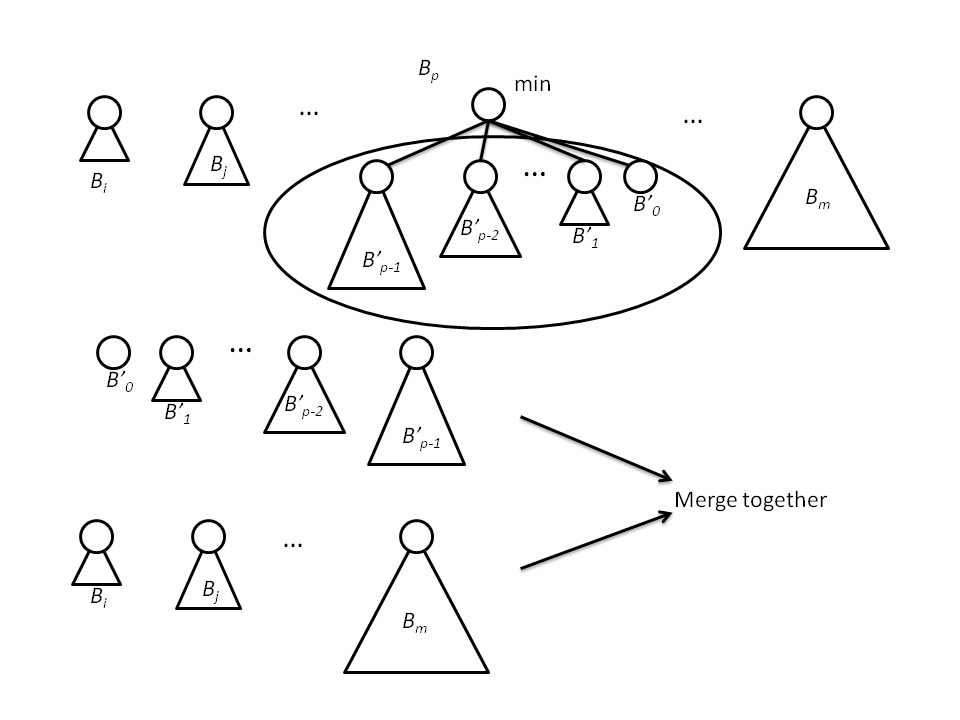
\includegraphics[scale=0.5]{img/bheap-pop.eps}
  \caption{Pop the minimum element from a binomial heap.}
  \label{fig:bheap-del-min}
\end{figure}

In order to realize this algorithm, we first need to define an
auxiliary function, which can extract the tree contains the minimum
element at root from the forest.

\be
removeMinT(H) = \left \{
  \begin{array}
  {r@{\quad:\quad}l}
  (T, \phi) & \text{H is a singleton as } \{ T \} \\
  (T_1, H') & Root(T_1) < Root(T') \\
  (T', \{T_1\} \cup H'') & otherwise  
  \end{array}
\right .
\ee

where

\[
  \begin{array}{lr}
  H = \{ T_1, T_2, ...\} & \text{for the non-empty forest case;} \\
  H' = \{ T_2, T_3, ...\} & \text{is the forest without the first tree;} \\
  (T', H'') = remvoeMinT(H')
  \end{array}
\]

The result of this function is a tuple. The first part is the 
tree which has the minimum element at root, the second part is
the rest of the trees after remove the first part from the forest.

This function examine each of the trees in the forest thus is bound
to $O(\lg N)$ time.

The relative Haskell program can be give respectively.

\lstset{language=Haskell}
\begin{lstlisting}
removeMinTree :: (Ord a) => BiHeap a -> (BiTree a, BiHeap a)
removeMinTree [t] = (t, [])
removeMinTree (t:ts) = if root t < root t' then (t, ts) 
                       else (t', t:ts')
    where
      (t', ts') = removeMinTree ts
\end{lstlisting}

With this funciton defined, to return the minimum element is trivial.

\begin{lstlisting}
findMin :: (Ord a) => BiHeap a -> a
findMin = root . fst. removeMinTree
\end{lstlisting}

Of course, it's possible to just traverse forest and pick the
minimum root without remove the tree for this purpose. Below
imperative algorithm describes it with `left child, right sibling' 
approach.

\begin{algorithmic}[1]
\Function{FIND-MINUMUM}{$H$}
  \State $T \gets HEAD(H)$
  \State $min \gets \infty$
  \While{$T \ne \phi$}
    \If{$KEY(T) < min$}
      \State $min \gets KEY(T)$
    \EndIf
    \State $T \gets SIBLING(T)$
  \EndWhile
  \State \Return $min$
\EndFunction
\end{algorithmic}

While if we manage the children with collection containers, the link
list traversing is abstracted as to find the minmum element among the list.
The following Python program shows about this situation.

\lstset{language=Python}
\begin{lstlisting}
def find_min(ts):
    min_t = min(ts, key=lambda t: t.key)
    return min_t.key
\end{lstlisting}

Next we define the function to delete the minimum element from
the heap by using $removeMinT$.

\be
delteMin(H) = merge(reverse(Children(T)), H')
\ee

where

\[
  (T, H') = removeMinT(H)
\]

Translate the formula to Haskell program is trivial and we'll skip
it.

To realize the algorithm in procedural way takes extra efforts
including list reversing etc. We left these details as exercise to the
reader. The following pseudo code illustrate the imperative 
pop algorithm

\begin{algorithmic}[1]
\Function{Extract-Min}{$H$}
  \State $(T_{min}, H) \gets$ \Call{Extract-Min-Tree}{$H$}
  \State $H \gets$ \textproc{Merge}($H$, \textproc{Reverse}(\Call{Children}{$T_{min}$}))
  \State \Return (\Call{Key}{$T_{min}$}, $H$)
\EndFunction
\end{algorithmic}

With pop operation defined, we can realize heap sort by creating
a binomial heap from a series of numbers, than keep popping the
smallest number from the heap till it becomes empty.

\be
sort(xs) = heapSort(fromList(xs))
\ee

And the real work is done in function $heapSort$.

\be
heapSort(H) = \left \{
  \begin{array}
  {r@{\quad:\quad}l}
  \phi & H = \phi \\
  \{ findMin(H)  \} \cup heapSort(deleteMin(H)) & otherwise
  \end{array}
\right .
\ee

Translate to Haskell yeilds the following program.

\lstset{language=Haskell}
\begin{lstlisting}
heapSort :: (Ord a) => [a] -> [a]
heapSort = hsort . fromList where
    hsort [] = []
    hsort h = (findMin h):(hsort $ deleteMin h)
\end{lstlisting} %$

Function fromList can be defined by folding. Heap sort can 
also be expressed in procedural way respectively. Please refer to 
previous chapter about binary heap for detail.

\subsubsection*{Exercise}
\begin{itemize}
\item Write the program to return the minimum element from a
binomial heap in your favorate imperative programming language
with 'left-child, right-sibling' approach.

\item Realize the \textproc{Extract-Min-Tree}() Algorithm.

\item For 'left-child, right-sibling' approach, reversing all
children of a tree is actually reversing a single-direct linked-list.
Write a program to reverse such linked-list in your favorate
imperative programming language.
\end{itemize}

\subsubsection{More words about binomial heap}
As what we have shown that insertion and merge are bound to $O(\lg N)$
time. The results are all ensure for the {\em worst case}. The 
armortized performance are $O(1)$. We skip the proof for this
fact.

% ================================================================
%                 Fibonacci heaps
% ================================================================
\section{Fibonacci Heaps}
\label{fib-heap}

It's interesting that why the name is given as `Fibonacci heap'.
In fact, there is no direct connection from the structure design
to Fibonacci series. The inventors of `Fibonacci heap', Michael L.
Fredman and Robert E. Tarjan, utilized the property of Fibonacci heap
to prove the performance time bound, so they decided to use Fibonacci
to name this data structure.\cite{CLRS} 

% ================================================================
%                 Definition
% ================================================================
\subsection{Definition}

Fibonacci heap is essentially a lazy evaluated binomial heap. Note
that, it doesn't mean implementing binomial heap in lazy evaluation
settings, for instance Haskell, brings Fibonacci heap automatically.
However, lazy evaluation setting does heap in realization. For example
in \cite{hackage-fibq}, presents a elegant implementation.

Fibonacci heap has excellent performance theoretically. All operations
except for pop are bound to amortized $O(1)$ time. In this section,
we'll give an algorithm different from some popular textbook\cite{CLRS}.
Most of the ideas present here are based on Okasaki's work\cite{okasaki-fibh}.

Let's review and compare the performance of binomial heap and Fibonacci
heap (more precisely, the performance goal of Fibonacci heap).

% \begin{table}
% \caption{Performance goal of Fibonacci heap}
\begin{tabular}{l | c | r}
  \hline
  operation & Binomial heap & Fibonacci heap \\
  \hline
  insertion & $O(\lg N)$ & $O(1)$ \\
  merge & $O(\lg N)$ & $O(1)$ \\
  top & $O(\lg N)$ & $O(1)$ \\
  pop & $O(\lg N)$ & amortized $O(\lg N)$ \\
  \hline
\end{tabular}
% \end{table}

Consider where is the bottleneck of inserting a new element $x$ to 
binomial heap. We actually wrap $x$ as a singleton leaf and merge
it to the heap. In the merge operation, we inserted the tree in 
monotically increasing order of rank, and once the rank is equal,
recursively linking and inserting will happen, which lead to the
$O(\lg N)$ time.

As the lazy strategy, we can postpone the ordered-rank insertion and
merging operations. On the contrary, we just drop the singleton
leaf to the forest. The problem is that when we try to find the
minimum element, for example the top operation, the performance
will be bad, because we need check all trees in the forest, and 
there aren't only $O(\lg N)$ trees any more.

In order to locate the top element in constant time, we must remember
where is the tree contains the minimum element as root.

Based on this idea, we can reuse the definition of binomial tree
and give the definition of Fibonacci heap as the following.

\lstset{language=Haskell}
\begin{lstlisting}
data BiTree a = Node { rank :: Int
                     , root :: a
                     , children :: [BiTree a]}
\end{lstlisting}

The Fibonacci heap is either empty or a forest of binomail trees with
the minimum element stored in a special one explicitly.

\begin{lstlisting}
data FibHeap a = E | FH { size :: Int
                        , minTree :: BiTree a
                        , trees :: [BiTree a]}
\end{lstlisting}

For convenient purpose, we also add a size field to record how many
elements are there in a heap.

% ================================================================
%          Basic Heap operations       
% ================================================================
\subsection{Basic heap operations}

\subsubsection{Find the minimum element in the heap (top)}

\subsubsection{Insert a new element to the heap}

\subsubsection{Merge two heaps}

\subsubsection{Extract the minimum element from the heap (pop)}

\subsubsection{Decrease an element}

\subsubsection{Delete an element}

\subsection{Running times}


% ================================================================
%                 Pairing Heaps
% ================================================================

\section{Pairing Heaps}
\label{pairing-heap}

% ================================================================
%                 Definition
% ================================================================
\subsection{Definition}

% ================================================================
%          Basic Heap operations       
% ================================================================
\subsection{Basic heap operations}

\subsubsection{Find the minimum element in the heap (top)}

\subsubsection{Insert a new element to the heap}

\subsubsection{Merge two heaps}

\subsubsection{Extract the minimum element from the heap (pop)}

\subsubsection{Decrease an element}

\subsubsection{Delete an element}

% ================================================================
%                 Short summary
% ================================================================
\section{Notes and short summary}

% ================================================================
%                 Appendix
% ================================================================
\section{Appendix} \label{appendix}
%\appendix
All programs provided along with this article are free for
downloading.

\subsection{Prerequisite software}
GNU Make is used for easy build some of the program. For C++ and ANSI C programs,
GNU GCC and G++ 3.4.4 are used. 
For Haskell programs GHC 6.10.4 is used
for building. For Python programs, Python 2.5 is used for testing, for
Scheme/Lisp program, MIT Scheme 14.9 is used.

all source files are put in one folder. Invoke 'make' or 'make all'
will build C++ Program. 

There is no separate Haskell main program module, however, it is possible to run the program in GHCi.

\begin{itemize}
\item files

\end{itemize}

download position: http://sites.google.com/site/algoxy/otherheaps/otherheaps.zip

\begin{thebibliography}{99}

\bibitem{K-ary-tree}
K-ary tree, Wikepedia. http://en.wikipedia.org/wiki/K-ary\_tree

\bibitem{CLRS}
Thomas H. Cormen, Charles E. Leiserson, Ronald L. Rivest and Clifford Stein. ``Introduction to Algorithms, Second Edition''. The MIT Press, 2001. ISBN: 0262032937.

\bibitem{okasaki-book}
Chris Okasaki. ``Purely Functional Data Structures''. Cambridge university press, (July 1, 1999), ISBN-13: 978-0521663502

\bibitem{wiki-pascal-triangle}
Wikipedia, ``Pascal's triangle''. http://en.wikipedia.org/wiki/Pascal's\_triangle

\bibitem{hackage-fibq}
Hackage. ``An alternate implementation of a priority queue based on a Fibonacci heap.'', http://hackage.haskell.org/packages/archive/pqueue-mtl/1.0.7/doc/html/src/Data-Queue-FibQueue.html

\bibitem{okasaki-fibh}
Chris Okasaki. ``Fibonacci Heaps.'' http://darcs.haskell.org/nofib/gc/fibheaps/orig

\end{thebibliography}

\ifx\wholebook\relax \else
\end{document}
\fi
